\chapter{Security of IP networks}

\begin{figure}[h]
    \centering
    \includegraphics[page = 2,trim = 0.7cm 2.2cm 0.7cm 4cm, clip, width = 0.55\textwidth]{\slides}
    \caption{Remote access via dial-up lines}
\end{figure}

%\paragraph*{Remote access via dial-up lines}
The first point regarding the security of IP networks involves \ul{controlling who can access the networks}.
In the past, it was primarily used for residential users who utilized a modem to connect to a telephone line (switched network).
This process involved transforming bits into sound and having equivalent equipment on the ISP side, which would accept the telephone call and convert it into network packets.
To facilitate this, devices known as \textbf{NAS} (\textit{Network Access Server}) were employed.
NAS had the responsibility of \underline{authenticating users}, \underline{performing access control}, and subsequently \underline{providing users with access} to the IP network - typically the internet, but in some cases also allowing access to a company's internal network from home.
Nowadays, this system is no longer widely used, at least in Western countries, although some countries still rely on it.


\begin{figure}[h]
    \centering
    \includegraphics[page = 3,trim = 0.7cm 2.2cm 0.7cm 3.7cm, clip, width = 0.55\textwidth]{\slides}
    \caption{Network access (modern way)}
\end{figure}

%\paragraph*{Network access (modern way)}
Today, it is possible to access the Internet in different ways, which basically depends on the device.
For example, a smartphone typically uses technologies such as 3G, 4G, or 5G to connect to the base station, which runs an \textbf{authentication protocol} with the \textbf{AAA server} to check if the user is authorized for an internet connection.
It is also possible to use Wi-Fi to connect to access points, which provide the translation from a wireless to a wired network and can again verify access.
Alternatively, there could be a home gateway, which provides access to the Internet using both Ethernet and Wi-Fi (only if properly authenticated).
In all these scenarios, authentication is always required before permitting traffic from a specific user.
Therefore, there is a difference between the \textit{local branch} / \textit{last mile}, \textit{border element}, and \textit{the core network}.



\section{Authentication of PPP channels}
There is a need to authenticate a user before enabling network transmission. The authentication process begins when someone attempts to connect, and at this point, the physical layer (Layer 1) for physical transmissions is already available. Since we are working at a logical level, Layer 2 (data layer connectivity) is also accessible.

On top of data layer connectivity, a protocol specific to transporting data is usually running. Typically, this protocol is \textbf{PPP} (\textit{Point-to-Point Protocol}), designed to \textbf{encapsulate network packets} such as Layer 3 (e.g., IP) and \textbf{carry them over a point-to-point link}. This PPP link can be a physical connection like an ISDN line or a telephone network; alternatively, it can be a virtual layer, as is the case when starting from a home gateway with access to ADSL using PPPoE (PPP over Ethernet) to transport packets between the home gateway and the provider.

Moreover, PPP is utilized to carry packets within virtualized Layer 3 connections with a specific and somewhat complex\footnote{The professor described it as "horrible"} protocol named L2TP (Layer 2 Tunnel Protocol). L2TP is a Layer 2 encapsulated inside UDP/IP (which is Layer 4), which deviates from the normal behaviors of a network.

Regardless, once PPP is enabled, numerous virtual point-to-point connections extend from the device to an access point. PPP activation occurs in three steps:

\begin{enumerate}
    \item \textbf{LCP (Link Control Protocol):} Establishes the ability to transmit data, and can also negotiate authentication protocols and algorithms.
    \item \textbf{Authentication (optional; PAP, CHAP, or EAP):} Performs user authentication.
    \item \textbf{L3 encapsulation:} Handles Layer 3 encapsulation via various \textbf{NCP}s (Network Control Protocols), such as IPCP (IP Control Protocol).
\end{enumerate}




\subsection{Authentication of a network access}
There are three methods to authenticate network access over PPP:

\begin{itemize}
    \item \textbf{PAP (Password Authentication Protocol):} This is the oldest method; in this case, the user sends the username and password in clear over the PPP channel. If someone is sniffing the channel, they can acquire the password.

    \item \textbf{CHAP (Challenge Handshake Authentication Protocol):} It uses a symmetric challenge-response based on the user's password. In this case, the password cannot be copied, but the channel is not protected. Instead of inventing other protocols tied to a specific authentication mechanism, a generalization has been made by introducing EAP.

    \item \textbf{EAP (Extensible Authentication Protocol):} It is a authentication framework that does not implement any specific method. The authentication method is external; for example, challenge-response, OTP, or TLS can be used.
\end{itemize}

Nowadays, PAP and CHAP should never be used, while EAP is the most widely adopted method for authenticating network access.

\subsection{LCP Authentication - Protocol
    Configuration Option}
If the Protocol Configuration Option in LCP Authentication exists, it includes several components:

\begin{itemize}
    \item \textbf{Type (8-bit):} Denotes the option type.
    \item \textbf{Length (8-bit):} Represents the length of the option in bytes.
    \item \textbf{Authentication Protocol (16-bit):} Specifies the protocol identifier.
    \item \textbf{[ Algorithm (8-bit) ]:} Optional field for algorithm identifier, required when a protocol supports various algorithms.

          For PAP (Password Authentication Protocol):
          \begin{itemize}
              \item \textbf{Type:} 3
              \item \textbf{Length:} 4
              \item \textbf{Protocol:} \texttt{0xC023}
          \end{itemize}

          For CHAP (Challenge Handshake Authentication Protocol):
          \begin{itemize}
              \item \textbf{Type:} 3
              \item \textbf{Length:} 5
              \item \textbf{Protocol:} \texttt{0xC223}
              \item \textbf{Algorithm:} 5 (for MD5)
          \end{itemize}
\end{itemize}


% NOTE: PAP and CHAP sections were added in 2023/24
\subsubsection{PAP}
\textbf{PAP}, or \textit{Password Authentication Protocol}, is defined in RFC-1334 "PPP Authentication Protocols" (Oct 1992). This RFC also introduces the initial version of CHAP. 

In PAP, the user-id and password are transmitted in clear text between the Peer and the Authenticator, posing a significant security risk. Authentication occurs only once when the channel is created, making it a potentially vulnerable method. Due to the clear transmission of sensitive information, PAP is considered very dangerous and is not recommended for secure network communication.

\paragraph{PAP: 2-way Handshake Protocol}
PAP employs a 2-way handshake protocol involving communication between the Peer and the Authenticator.

\begin{itemize}
    \item ($Peer \rightarrow Authenticator$) \texttt{Authenticate-Request} ($code=1$)
    \begin{itemize}
        \item Code (8-bit) + Identifier (8-bit) + Length (16-bit)
        \item Peer-ID Length (8-bit) + Peer-ID (0-255B)
        \item Passwd-Length (8-bit) + Password (0-255B)
    \end{itemize}
    \item ($Authenticator \rightarrow Peer$) \texttt{Authenticate-Response} ($code= 2, 3$)
    \begin{itemize}
        \item Code (8-bit) + Identifier (8-bit) + Length (16-bit)
        \item Msg-Length (8-bit) + Message (0-255B)
        \item Code=2 (ACK), Code=3 (NAK)
    \end{itemize}
\end{itemize}

An identifier is essential for correlating the \texttt{Authenticate-Request} with its corresponding \texttt{Authenticate-Response}. Given the potential loss of either loss of either request or response, it becomes imperative for the Authenticator to accommodate multiple requests. Therefore, to mitigate the risk of lost messages, the Authenticator \textbf{MUST} allow for the submission of multiple \texttt{Authenticate-Request} or \texttt{Authenticate-Response} messages.
This identifier is also pivotal in preventing replay attacks. Without it, an adversary could intercept and replay the message, potentially granting unauthorized access.



\subsubsection{CHAP}
\textbf{CHAP}, or \textit{Challenge Handshake Authentication Protocol}, is defined in RFC-1994 "PPP Challenge Handshake Authentication Protocol (CHAP)" (Aug 1996). It introduces a symmetric challenge (password-based) authentication mechanism. 

In CHAP, the initial challenge is compulsory and occurs at channel creation. The authentication request can optionally be repeated, with a different challenge, during transmission. The decision to repeat the authentication request is taken by the Network Access Server (NAS). It's important to note that the challenge MUST be a nonce.

For systems supporting both PAP and CHAP, the Authenticators must offer CHAP as the preferred authentication method.

\paragraph{CHAP: 3-way Handshake Protocol}
CHAP employs a 3-way handshake protocol involving communication between the Authenticator and the Peer.
\underline{After the link is established}:

\begin{itemize}
    \item ($Authenticator \rightarrow Peer$) \texttt{Challenge} ($code=1$)
    \begin{itemize}
        \item Code (8-bit) + Identifier (8-bit) + Length (16-bit)
        \item Challenge-Size (8-bit) + Challenge-Value (0-255B)
    \end{itemize}
    \item ($Peer \rightarrow Authenticator$) \texttt{Response} ($code=2$)
    \begin{itemize}
        \item Code (8-bit) + Identifier (8-bit) + Length (16-bit)
        \item Response-Size (8-bit) + Response-Value (0-255B)
    \end{itemize}
    \item ($Authenticator \rightarrow Peer$) \texttt{Result} ($code= 3$ Success, $4$ Failure)
    \begin{itemize}
        \item Code (8-bit) + Identifier (8-bit) + Length (16-bit)
    \end{itemize}
\end{itemize}

\textit{Response-Value} is calculated using \texttt{md5(Identifier || pwd || Challenge-Value)} (in the version specified in 1996). The server checks the response by comparing it with its own calculation of the expected hash value. If the values match, the authentication is acknowledged; otherwise, the connection is usually terminated.

The identifier is crucial for correlating the Request and Response. In case of lost \texttt{Challenge} or \texttt{Response}, the Authenticator \textbf{MUST} resend the Challenge until the retry limit is reached.



\subparagraph*{Packet Loss in PPP Implementation}
One interesting point to consider is the idea that challenges or responses could be lost in a PPP (point-to-point protocol). You might wonder why, especially when we have a direct connection between two peers using an Ethernet cable or Wi-Fi. Usually, in such direct connections, we expect very little or no loss of information.

The confusion arises due to the varied ways PPP can be used. We mentioned earlier that PPP can operate on different types of transport, including a virtual setup within UDP. Here's the catch: UDP, unlike other more reliable protocols, doesn't ensure that your data reaches its destination every time. Moreover, UDP is built on top of IP, which also doesn't guarantee that your information will be reliably delivered.

This becomes apparent when we consider how PPP packets are implemented in real-world situations. In some cases, instead of sticking to the logical layering (PPP being at layer 2), PPP packets may be placed inside layer 4 due to certain implementation choices. This might seem like a strange decision, but it happens. As a result, even though you might think a direct point-to-point connection is rock-solid, these implementation choices could lead to some data loss. So, when designing such protocols, it's crucial to account for all possible scenarios, even the ones that might seem unlikely at first.


\paragraph{MS-CHAP}
MS-CHAP, or Microsoft PPP CHAP Extensions, is a set of protocols developed by Microsoft to enhance the functionality of the Challenge Handshake Authentication Protocol (CHAP) in PPP connections\footnote{"The usual approach from Microsoft, in which they take something standard and make it non-standard".}.


\begin{itemize}
    \item \textbf{MS-CHAPv1:}
    \begin{itemize}
        \item RFC 2433 "Microsoft PPP CHAP Extensions" (October 1998).
        \item Initially included but later discontinued by Microsoft starting with Windows Vista.
    \end{itemize}
    
    \item \textbf{MS-CHAPv2:}
    \begin{itemize}
        \item RFC 2759 "Microsoft PPP CHAP Extensions, v2" (January 2000).
        \item Continued the evolution of MS-CHAP, dropped by Microsoft starting with Windows 11 22H2.
    \end{itemize}
\end{itemize}

LCP negotiates the CHAP algorithm, with \texttt{0x80} for MS-CHAPv1 and \texttt{0x81} for MS-CHAPv2, using option 3 (Authentication Protocol).

MS-CHAP is a Microsoft-specific implementation of CHAP concepts.
Despite its origin, MS-CHAP is supported by many other vendors, including CISCO.


\subparagraph{MS-CHAP: Extensions over CHAP}
MS-CHAP extends the principles of CHAP but operates as a distinct protocol with unique features.

\begin{itemize}
    \item \textbf{Common Features (v1 and v2):}
    \begin{itemize}
        \item Authenticator-controlled password change.
        \item Authenticator-controlled authentication retry.
        \item Specific failure codes.
    \end{itemize}

    \item \textbf{MS-CHAPv2 Mutual Authentication:}
    \begin{itemize}
        \item Achieved by piggybacking a peer challenge on the Response packet.
        \item Includes an authenticator response on the Success packet.
    \end{itemize}
\end{itemize}

In order to implement this protocol, each peer must know the plaintext password or an MD4 hash of the password. Note: This approach is not compatible with most password storage formats.


\begin{figure}[H]
    \centering
    \includegraphics[page = 13,trim = 0.5cm 2.2cm .5cm 4cm, clip, width = .70\textwidth]{\slides}
    \caption{The MS-CHAPv2 protocol}
\end{figure}

\begin{figure}[H]
    \centering
    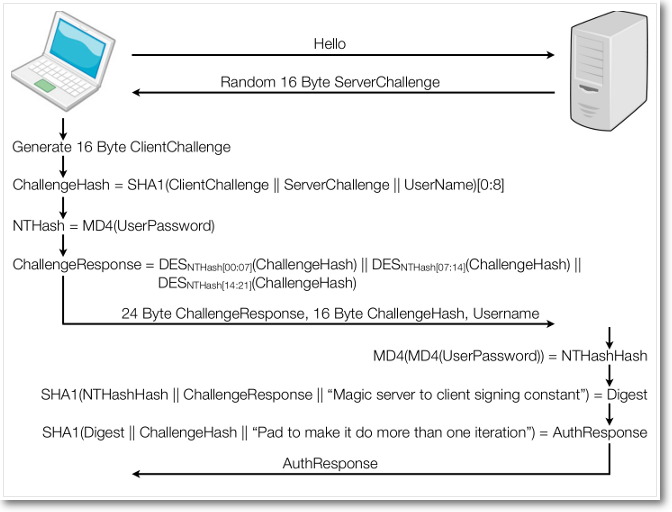
\includegraphics[width = .70\textwidth]{chapter4/MS-CHAPv2.png}
    \caption{MS-CHAPv2 - Another frame of reference. Please consider the professor's slide. Taken from\\ 
    \url{https://web.archive.org/web/20160316174007/https://www.cloudcracker.com/blog/2012/07/29/cracking-ms-chap-v2/}}
\end{figure}


\subparagraph{MS-CHAPv2: an attack}
MS-CHAPv2, once deemed a secure authentication protocol, is susceptible to a specific attack exploiting a known ciphertext-plaintext pair denoted as \(R\) and \(H\). The primary objective is to decipher the three keys, namely \(K_{0-6}\), \(K_{7-13}\), and \(K_{14-20}\). Directly employing a brute-force approach on the password is considered impractical due to the significant time involved. Alternatively, a brute-force attack on the keys poses a challenge, requiring approximately \(2^{56} + 2^{56} + 2^{56}\) operations.

However, it's crucial to note that \(K\) is only 128 bits (MD4 output), i.e., 16 bytes, and \(K_{14-20}\) has only two bytes (\(K_{14-15}\)) padded with zeros. To find \(K_{14-20}\), \(2^{16}\) operations are needed. The process involves \(2^{56}\) operations to find \(K_{0-6}\) and \(K_{7-13}\), followed by a comparison with \(R1\) and \(R2\). Utilizing a divide-and-conquer strategy reduces the effort to approximately \(2^{56}\) operations (less than 23 hours with DES FPGA).

\begin{figure}[H]
    \centering
    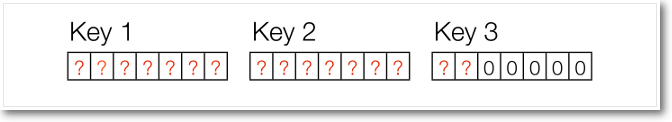
\includegraphics[width = .70\textwidth]{chapter4/MS-CHAPv2_attack1.png}
    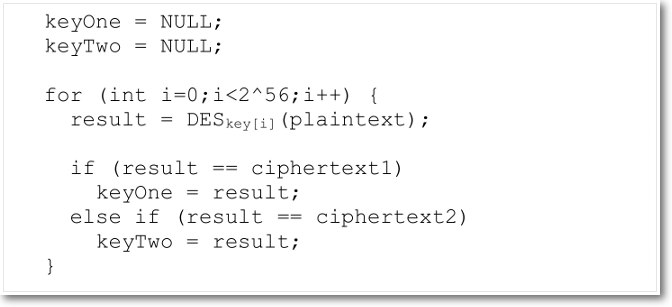
\includegraphics[width = .70\textwidth]{chapter4/MS-CHAPv2_attack2.png}
\end{figure}

In conclusion, MS-CHAPv2 should NEVER be used anymore and has been officially deprecated, including its removal in Windows 11 22H2.
